\PassOptionsToPackage{unicode=true}{hyperref} % options for packages loaded elsewhere
\PassOptionsToPackage{hyphens}{url}
%
\documentclass[ignorenonframetext,]{beamer}
\usepackage{pgfpages}
\setbeamertemplate{caption}[numbered]
\setbeamertemplate{caption label separator}{: }
\setbeamercolor{caption name}{fg=normal text.fg}
\beamertemplatenavigationsymbolsempty
% Prevent slide breaks in the middle of a paragraph:
\widowpenalties 1 10000
\raggedbottom
\setbeamertemplate{part page}{
\centering
\begin{beamercolorbox}[sep=16pt,center]{part title}
  \usebeamerfont{part title}\insertpart\par
\end{beamercolorbox}
}
\setbeamertemplate{section page}{
\centering
\begin{beamercolorbox}[sep=12pt,center]{part title}
  \usebeamerfont{section title}\insertsection\par
\end{beamercolorbox}
}
\setbeamertemplate{subsection page}{
\centering
\begin{beamercolorbox}[sep=8pt,center]{part title}
  \usebeamerfont{subsection title}\insertsubsection\par
\end{beamercolorbox}
}
\AtBeginPart{
  \frame{\partpage}
}
\AtBeginSection{
  \ifbibliography
  \else
    \frame{\sectionpage}
  \fi
}
\AtBeginSubsection{
  \frame{\subsectionpage}
}
\usepackage{lmodern}
\usepackage{amssymb,amsmath}
\usepackage{ifxetex,ifluatex}
\usepackage{fixltx2e} % provides \textsubscript
\ifnum 0\ifxetex 1\fi\ifluatex 1\fi=0 % if pdftex
  \usepackage[T1]{fontenc}
  \usepackage[utf8]{inputenc}
  \usepackage{textcomp} % provides euro and other symbols
\else % if luatex or xelatex
  \usepackage{unicode-math}
  \defaultfontfeatures{Ligatures=TeX,Scale=MatchLowercase}
\fi
\usetheme[]{Warsaw}
\usecolortheme{beaver}
% use upquote if available, for straight quotes in verbatim environments
\IfFileExists{upquote.sty}{\usepackage{upquote}}{}
% use microtype if available
\IfFileExists{microtype.sty}{%
\usepackage[]{microtype}
\UseMicrotypeSet[protrusion]{basicmath} % disable protrusion for tt fonts
}{}
\IfFileExists{parskip.sty}{%
\usepackage{parskip}
}{% else
\setlength{\parindent}{0pt}
\setlength{\parskip}{6pt plus 2pt minus 1pt}
}
\usepackage{hyperref}
\hypersetup{
            pdftitle={Homework \#3},
            pdfauthor={Brendan Case},
            pdfborder={0 0 0},
            breaklinks=true}
\urlstyle{same}  % don't use monospace font for urls
\newif\ifbibliography
\setlength{\emergencystretch}{3em}  % prevent overfull lines
\providecommand{\tightlist}{%
  \setlength{\itemsep}{0pt}\setlength{\parskip}{0pt}}
\setcounter{secnumdepth}{0}

% set default figure placement to htbp
\makeatletter
\def\fps@figure{htbp}
\makeatother


\title{Homework \#3}
\author{Brendan Case}
\date{9/12/2018}

\begin{document}
\frame{\titlepage}

\begin{frame}{Slide with Bullet (Stings)}
\protect\hypertarget{slide-with-bullet-stings}{}

Here are some insects with some spicy stings:

\begin{itemize}
\tightlist
\item
  \color{blue} Sweat Bee
\item
  \color{yellow} Bald-faced Hornet
\item
  \color{orange} Red Paper Wasp
\item
  \color{red} Bullet Ant
\end{itemize}

\end{frame}

\begin{frame}{Incremental Bullets + Bigskip}
\protect\hypertarget{incremental-bullets-bigskip}{}

\begin{itemize}[<+->]
\tightlist
\item
  There is one sting which is even spicier\ldots{}.
\item
  **drumroll** \bigskip \bigskip \bigskip \bigskip
\item
  \textit{Synoeca septentrionalis}!! \only<3>{
  \begin{picture}(320,250)
  \put(200,170){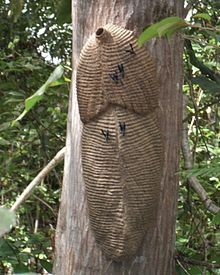
\includegraphics[height=4cm]{warriorwasp.jpg}}
  \put(60,120){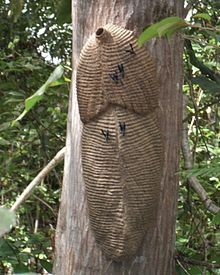
\includegraphics[height=4cm]{warriorwasp.jpg}}
  \end{picture}}
\end{itemize}

\end{frame}

\begin{frame}{Figure In \LaTeX~Using Centering}
\protect\hypertarget{figure-in-using-centering}{}

\begin{center}
 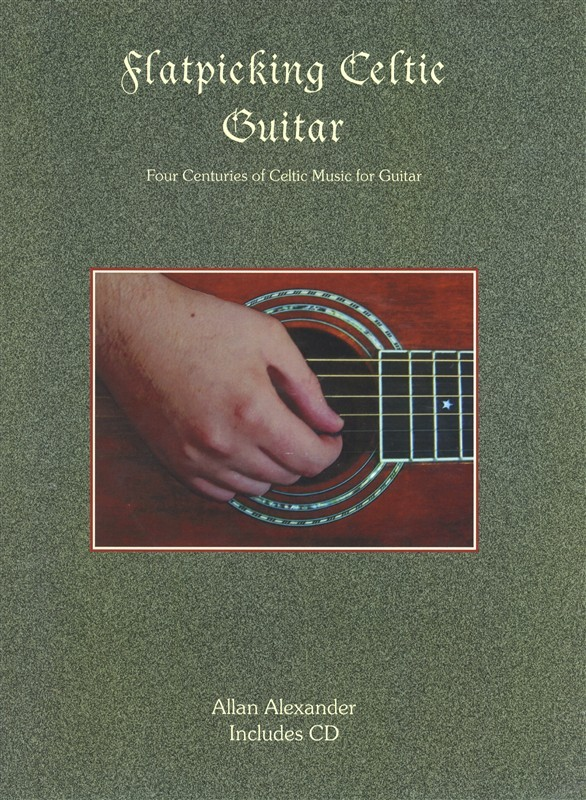
\includegraphics[height=6cm]{celtic.jpg}
 \end{center}

Often, putting an image in a center environment is easiest.

\end{frame}

\begin{frame}{Figure In \LaTeX~Using Minipages}
\protect\hypertarget{figure-in-using-minipages}{}

\begin{picture}(320,250)
 \put(5,50){
\includegraphics[height=5.5cm]{blackboard.png}}
 \put(95,180){\begin{minipage}[t]{0.4\linewidth}
 {\color{white} Choose a point on the unit circle. Connect it to the origin with a line of length one, and denote the angle between that line and the horizontal coordinate axis by $\theta$.}
 \end{minipage}}
 \end{picture}

\end{frame}

\end{document}
